\documentclass[11pt]{article}
\usepackage[margin=1in]{geometry}
\usepackage{amsmath,amssymb,amsthm}
\usepackage{booktabs}
\usepackage{caption}
\usepackage{float}
\usepackage{graphicx}
\usepackage{xcolor}
\usepackage{microtype}
\usepackage{hyperref}
\usepackage{url}

\hypersetup{colorlinks=true,linkcolor=blue!55!black,citecolor=blue!55!black,urlcolor=blue!55!black}
\captionsetup{font=small,labelfont=bf}
\setlength{\tabcolsep}{5pt}
\emergencystretch=2em

\newtheorem{theorem}{Theorem}[section]
\newtheorem{proposition}[theorem]{Proposition}
\newtheorem{lemma}[theorem]{Lemma}
\newtheorem{corollary}[theorem]{Corollary}
\theoremstyle{definition}
\newtheorem{definition}[theorem]{Definition}
\newtheorem{remark}[theorem]{Remark}

\newcommand{\R}{\mathbb{R}}
\newcommand{\norm}[1]{\left\lVert #1\right\rVert}
\newcommand{\spec}{\operatorname{spec}}
\newcommand{\spr}{\varrho}
\newcommand{\diag}{\operatorname{diag}}
\newcommand{\argmin}{\operatorname*{arg\,min}}
\newcommand{\Id}{\mathrm{I}}
\newcommand{\Ufour}{U_{\mathrm{4C}}}
\newcommand{\Upatch}{U_{\mathrm{patch}}}

\title{\textbf{Four-Corner Spectral Tuning for Quadratic ADMM\\
with Application to Diffeomorphic Image Registration}}
\author{Katherine Xie \qquad Jie Wu \qquad
Xiaohui Xie\thanks{Corresponding author:
\href{mailto:xhx@uci.edu}{xhx@uci.edu}.}\\
\normalsize Department of Computer Science, University of California, Irvine,
Irvine, California, USA}
\date{}

\begin{document}
\maketitle

\begin{abstract}
Selecting the penalty and relaxation parameters of the alternating direction
method of multipliers (ADMM) can require repeated spectral-radius evaluation
of a large parameter-dependent iteration operator. We consider over-relaxed
ADMM (oADMM) for a separable quadratic split whose attained joint modal
spectrum is a Cartesian product of data and regularizer curvatures. The modal
contraction factor is monotone along each curvature coordinate line;
consequently, its largest magnitude is attained among four endpoint
combinations. The relaxation
parameter is optimized analytically for each penalty, and the remaining
penalty problem reduces to a finite algebraically characterized superset of
candidate minimizers. In this sense the method is search-free: it avoids
grid-based or iterative numerical optimization over the penalty while still
computing the required polynomial roots numerically. Full diffeomorphic image
registration is spatially varying and noncommuting, so the exact theorem does
not apply to the assembled operator. Coefficient freezing and the rank-one
optical-flow Hessian nevertheless yield an inexpensive predictor determined by
the four combinations of $h_-$, $h_+$, $g_-$, and $g_+$. On 134 FIRE retinal
pairs at $256\times256$, one-shot tuning reduced median pairwise runtime by
34.4\% and inner iterations by 39.6\% relative to a fixed pair selected on
separate validation data. On ten CIMA histology pairs, runtime decreased by
20.1\%. In both studies, landmark accuracy was essentially unchanged and no
nonpositive discrete Jacobian was observed.
\end{abstract}

\noindent\textbf{Keywords:} alternating direction method of multipliers;
parameter selection; spectral analysis; diffeomorphic image registration;
local Fourier analysis

\section{Introduction}\label{sec:introduction}
Spectral parameter selection for quadratic ADMM can be expensive in its own
right. For a trial penalty $\rho$, a spectral method constructs or applies the
corresponding iteration operator, estimates its convergence factor, and
repeats this calculation while optimizing $\rho$; over-relaxation introduces
the additional parameter $\alpha$. In large imaging systems the operator may
have hundreds of thousands of unknowns, so repeated spectral-radius evaluation
can offset the computational advantage of splitting. This issue is especially
pronounced after spatially varying image terms are assembled and whenever
relinearization changes the local Hessian.

The structural question addressed here is whether this spectral optimization
can collapse analytically when the quadratic operators possess separable modal
structure. For the class studied below, the oADMM contraction of a common mode
depends only on a data curvature $h$ and a regularizer curvature $g$. For fixed
$\rho$, this scalar factor is monotone along each coordinate line, with the
direction determined by the other curvature. If the
attained joint modal spectrum is the Cartesian product of the two curvature
sets, the worst contraction must therefore occur among
\[
(h_-,g_-),\quad(h_-,g_+),\quad(h_+,g_-),\quad(h_+,g_+).
\]
The large spectral optimization is reduced exactly to four rational scalar
branches. The optimal relaxation is available in closed form for each
penalty, and the reduced penalty objective is piecewise rational. Its global
minimum on a prescribed compact interval belongs to a finite algebraically
characterized candidate set.

We call this parameter selection \emph{search-free}: it performs neither a
grid search nor an iterative numerical optimization over $\rho$. Polynomial
roots in the finite candidate construction are still evaluated numerically;
the distinction is the replacement of repeated optimization and
spectral-radius evaluation by a fixed algebraic reduction.

The exact result requires more than commutativity. Simultaneous
diagonalization supplies paired eigenvalues $(h_i,g_i)$, but these pairs need
not fill the Cartesian product of the marginal spectra. The four endpoint
combinations are exact modes only under the separability and attainment
assumptions stated in Theorem~\ref{thm:fourcorner}. For arbitrary commuting
operators they define a rectangular envelope, and for noncommuting operators
they define a surrogate unless an independent bound is available.

Diffeomorphic image registration provides the motivating noncommuting
application. Its linearized data Hessian varies by pixel, whereas the Sobolev
regularizer couples neighboring pixels; the assembled matrices therefore
generally do not commute. Freezing the image coefficient recovers the separable
model locally. Moreover, each optical-flow Hessian is a rank-one update of a
multiple of the identity, so all required data curvature information reduces
to
\[
h_-=\nu,\qquad h_+=\nu+\mu\max_i\norm{\nabla I(x_i)}^2.
\]
Together with the regularizer endpoints $g_-$ and $g_+$, these values yield a
four-branch predictor after one $O(n)$ scan of gradient magnitudes. The result
is exact for the frozen separable family and predictive for the full
variable-coefficient registration operator.

The mathematical and computational progression is
\begin{align*}
\text{quadratic ADMM}&\longrightarrow\text{modal factor}
\longrightarrow\text{four corners}\\
&\longrightarrow\text{finite parameter selection}
\longrightarrow\text{noncommuting registration}.
\end{align*}

The contributions are:
\begin{enumerate}
\item A four-corner spectral theorem for quadratic oADMM under an attained
Cartesian-product joint modal spectrum.
\item A finite algebraic joint selection of $\rho$ and $\alpha$ that eliminates
grid-based or iterative penalty search for this structured model.
\item A registration specialization based on local coefficient freezing and
the rank-one optical-flow Hessian, reducing the data-term information required
for tuning to endpoint curvatures.
\item Experimental evidence that the surrogate-optimal parameters transfer to
noncommuting registration systems, reducing iterations and runtime while
maintaining landmark accuracy and observed topology.
\end{enumerate}

\section{Related Work}\label{sec:related}
\subsection{ADMM parameter selection}
Scaled ADMM and its practical residual criteria were systematized by Boyd
et al.\ \cite{Boyd2011}. Ghadimi et al.\ derived optimal parameters for
specific quadratic classes \cite{Ghadimi2015}. Teixeira et al.\ connected
parameter selection with scaling and constraint preconditioning in distributed
quadratic programs \cite{Teixeira2016}, while Giselsson and Boyd developed
tight contraction bounds that depend on the chosen metric
\cite{GiselssonBoyd2017}. These works obtain strong conclusions from particular
quadratic structure or operator bounds. The present analysis instead
identifies a joint modal structure under which the full worst-mode calculation
reduces to four attained endpoint pairs.

Adaptive methods avoid an offline spectral model. Residual balancing changes
the penalty according to primal and dual residual magnitudes
\cite{Wohlberg2017}; Barzilai--Borwein (BB) spectral updates estimate local
curvature from iterate differences \cite{Xu2017}. Such rules apply beyond the
separable setting considered here, but they update parameters from the
observed iteration history rather than solving the fixed quadratic model's
spectral minimax problem algebraically.

\subsection{Spectral and over-relaxed ADMM}
Song et al.\ address a broader class of linear-quadratic ADMM problems and
numerically optimize the spectral convergence factor with respect to the
penalty \cite{Song2024}. For each candidate $\rho$, their formulation requires
spectral information from the corresponding iteration operator; the
relaxation parameter is then selected conditionally. This generality is
valuable because it does not require the Cartesian-product modal structure
used here.

Direct application to full-resolution registration is computationally
demanding: the assembled variable-coefficient operator is large and
noncommuting, and its spectrum changes when image warping changes the
linearized Hessian. Repeated spectral-radius evaluation across trial penalties
can therefore make parameter selection expensive. A downsampled operator
reduces this cost but introduces a transfer problem between the coarse
spectral model and the full-resolution solve. The present work adopts the
complementary tradeoff. Stronger separability assumptions collapse the
structured spectral problem to four scalar branches and a finite penalty
candidate set; the resulting construction is then used as an inexpensive
predictor outside that exact class.
A coarse direct-spectral diagnostic illustrating this overhead and transfer
issue is reported in the supplementary information.

\subsection{Fourier and local Fourier analysis}
Fourier analysis has long characterized stationary iterations for elliptic
problems \cite{ChanElman1989}, and local Fourier analysis (LFA) is a standard
tool for multigrid design and parameter optimization
\cite{WienandsJoppich2005}. Translation-invariant periodic problems admit exact
Fourier decompositions; local and nonstandard analyses can remain informative
for random or discontinuous coefficients \cite{Rodrigo2017,Kumar2019}. Here the
stationary map is an ADMM error iteration, and local freezing converts a
matrix-valued optical-flow coefficient into a separable patch model.

\subsection{Variational image registration}
DARTEL \cite{Ashburner2007}, diffeomorphic demons
\cite{Vercauteren2009}, and large-deformation optimal-control formulations
\cite{MangBiros2015} are representative optimization-based registration
methods. Thorley et al.\ compose nonstationary velocity updates and solve
regularized convex subproblems with accelerated ADMM on graphics processing
units (GPUs)
\cite{Thorley2021}. Song et al.\ use a related quadratic model in their spectral
oADMM study \cite{Song2024}. Learning-based methods broaden the current
landscape \cite{Hering2022}, but the present work concerns numerical parameter
selection for the linearized variational subproblem.

\section{Quadratic ADMM and Reduced Error Dynamics}\label{sec:quadratic}
\subsection{Quadratic splitting}
Consider
\begin{equation}
\min_{v,w}\;
\underbrace{\tfrac12v^\top Hv+b^\top v}_{f(v)}
+\underbrace{\tfrac12w^\top Gw}_{r(w)}
\quad\text{subject to}\quad v-w=0,
\label{eq:split}
\end{equation}
where $v,w,b\in\R^N$ and $H,G\in\R^{N\times N}$ are symmetric positive
semidefinite matrices. The linear term $b$ determines the fixed point but
disappears from homogeneous error propagation.

\subsection{Standard and over-relaxed ADMM}
With scaled dual variable $u$ and penalty $\rho>0$, standard ADMM is
\begin{align}
(H+\rho\Id)v^{k+1}&=-b+\rho(w^k-u^k),\label{eq:vupdate}\\
(G+\rho\Id)w^{k+1}&=\rho(v^{k+1}+u^k),\label{eq:wupdate}\\
u^{k+1}&=u^k+v^{k+1}-w^{k+1}.\label{eq:uupdate}
\end{align}
For over-relaxed ADMM, abbreviated \emph{oADMM}, define
\begin{equation}
\widehat v^{k+1}=\alpha v^{k+1}+(1-\alpha)w^k,
\qquad 0<\alpha\le2,
\label{eq:relaxation}
\end{equation}
and replace $v^{k+1}$ by $\widehat v^{k+1}$ in
\eqref{eq:wupdate} and the dual update.

\subsection{Reduced Cayley representation}
The original oADMM recurrence couples primal and dual errors. Reducing it to
one $N$-dimensional operator isolates all dependence on $\rho$ and $\alpha$ and
exposes the common-mode scalar factor used in the four-corner argument. Define
\[
C_H(\rho)=(H-\rho\Id)(H+\rho\Id)^{-1},\qquad
C_G(\rho)=(G-\rho\Id)(G+\rho\Id)^{-1}.
\]
\begin{proposition}[Reduced Cayley error operator]\label{prop:reduced}
The nonzero spectra of the oADMM state map and
\begin{equation}
E_{\rho,\alpha}
=\left(1-\frac{\alpha}{2}\right)\Id
+\frac{\alpha}{2}C_H(\rho)C_G(\rho).
\label{eq:Ealpha}
\end{equation}
coincide, including algebraic multiplicity; the remaining state-map
eigenvalues are zero. Thus the asymptotic factor is
$\spr(E_{\rho,\alpha})$, where $\spr(\,\cdot\,)$ denotes the spectral radius
of a matrix or linear operator.
\end{proposition}
Appendix~\ref{app:reduced} gives the reduction. It is supporting machinery:
the parameter reduction below comes from the modal dependence of
\eqref{eq:Ealpha}.

\begin{theorem}[Basic contraction]\label{thm:contraction}
If $H,G\succeq0$ and $H+G\succ0$, then for every $\rho>0$,
$\kappa_\rho:=\norm{C_H(\rho)C_G(\rho)}_2<1$. Consequently
\[
\spr(E_{\rho,\alpha})
\le 1-\frac{\alpha}{2}(1-\kappa_\rho)<1,
\]
for $0<\alpha\le2$.
\end{theorem}
\begin{proof}
For $A\succeq0$, orthogonal diagonalization shows
$\norm{C_A(\rho)}_2\le1$, with norm preservation possible only on $\ker A$.
If a unit vector $x$ satisfied $\norm{C_HC_Gx}_2=1$, equality throughout
$\norm{C_HC_Gx}_2\le\norm{C_Gx}_2\le1$ would give
$x\in\ker G$ and $C_Gx=-x\in\ker H$. Hence
$x\in\ker H\cap\ker G$, contradicting $H+G\succ0$. The continuous function
$x\mapsto\norm{C_HC_Gx}_2$ attains its maximum on the finite-dimensional unit
sphere, so $\kappa_\rho<1$. Finally, the triangle inequality applied to
\eqref{eq:Ealpha} gives the stated bound.
\end{proof}

\paragraph{Nullspaces.}
If a nonzero vector lies in $\ker H\cap\ker G$, then
$C_HC_Gx=x$ and $E_{\rho,\alpha}x=x$ for every admissible parameter pair.
Strict contraction therefore requires $H+G\succ0$, or restriction to the
identifiable subspace. In the four-corner registration model,
$\nu=\gamma=0$ creates the $(h,g)=(0,0)$ mode; the selector then requires
positive damping, a coercive boundary/regularization condition, or explicit
removal of that common nullspace.

\subsection{Scalar modal factor}
When a vector is a common eigenvector of $H$ and $G$, with eigenvalues $h$ and
$g$, \eqref{eq:Ealpha} acts by
\begin{align}
e(h,g;\rho,\alpha)
&=1-\frac{\alpha}{2}
+\frac{\alpha}{2}
\frac{h-\rho}{h+\rho}\frac{g-\rho}{g+\rho}\label{eq:modal}\\
&=1-\alpha+\alpha\theta(h,g;\rho),\nonumber\\
\theta(h,g;\rho)&=
\frac{\rho^2+hg}{(\rho+h)(\rho+g)}.\label{eq:theta}
\end{align}
For nonnegative $h$ and $g$, $0\le\theta\le1$. The paired values $(h,g)$,
not the marginal spectra separately, determine the true modal factor.

\section{Four-Corner Spectral Tuning}\label{sec:fourcorner}
\subsection{Separable commuting modal structure}
\begin{definition}[Cartesian-product joint modal spectrum]\label{def:cartesian}
A quadratic split is \emph{separable} on modal sets
$\mathcal H$ and $\mathcal G$ if $H$ and $G$ are simultaneously diagonalizable
and their attained joint modal spectrum is
\[
\{(h,g): Hx=hx,\ Gx=gx\text{ for a common mode }x\ne0\}
=\mathcal H\times\mathcal G.
\]
For example,
$H_{\rm sep}=I_m\otimes H_c$ and
$G_{\rm sep}=G_s\otimes I_d$ have modes
$\phi_\xi\otimes z_j$ and pairs $(h_j,g(\xi))$, where
$H_cz_j=h_jz_j$, $G_s\phi_\xi=g(\xi)\phi_\xi$,
$H_c\in\R^{d\times d}$ acts on components,
$G_s\in\R^{m\times m}$ acts on spatial degrees of freedom, and $I_m,I_d$ are
the corresponding identity matrices.
\end{definition}
The Cartesian-product condition is stronger than commutativity. It asserts
that data and regularizer modes combine independently.

\subsection{Four-corner theorem}
For fixed $\rho>0$,
\begin{equation}
\frac{\partial\theta}{\partial h}
=\frac{\rho(g-\rho)}{(g+\rho)(h+\rho)^2},\qquad
\frac{\partial\theta}{\partial g}
=\frac{\rho(h-\rho)}{(h+\rho)(g+\rho)^2}.
\label{eq:theta_derivatives}
\end{equation}
The sign of the first derivative is independent of $h$, and the sign of the
second is independent of $g$. Thus, for fixed $\rho$, $\theta$ is monotone
along each coordinate line, although the direction may depend on the other
coordinate. Its minimum and maximum are therefore attained at corners.
Relaxation maps $\theta$ affinely to
$1-\alpha+\alpha\theta$; taking absolute value produces a convex function of
$\theta$, whose maximum over an interval is again attained at an endpoint.

\begin{theorem}[Four-Corner Spectral Theorem]\label{thm:fourcorner}
Suppose the joint modal spectrum is the Cartesian product
$\mathcal H\times\mathcal G$, where
$\mathcal H\subset[h_-,h_+]$ and
$\mathcal G\subset[g_-,g_+]$, with
$0\le h_-\le h_+$ and $0\le g_-\le g_+$. If all four endpoint combinations
are attained,
then
\begin{equation}
\spr(E_{\rho,\alpha})=
\Ufour(\rho,\alpha):=
\max_{\substack{h\in\{h_-,h_+\}\\g\in\{g_-,g_+\}}}
|e(h,g;\rho,\alpha)|
\label{eq:fourcorner}
\end{equation}
for every $\rho>0$ and $0<\alpha\le2$. If only the interval enclosure is known,
the right-hand side remains a valid rectangular upper envelope, but equality
with the true spectral radius need not hold.
\end{theorem}
\begin{proof}
Equation~\eqref{eq:theta_derivatives} makes the extrema of $\theta$ on the
rectangle occur at corners. The map
$t\mapsto|1-\alpha+\alpha t|$ is convex, so its maximum over the interval
between those extrema also occurs at an endpoint and hence at a corner.
Cartesian-product structure and attained endpoint combinations make those
corners actual modes, proving equality.
\end{proof}

\subsection{Optimal relaxation for fixed penalty}
Let the four corner values satisfy
\[
a(\rho)=\min_c\theta_c(\rho),\qquad
b(\rho)=\max_c\theta_c(\rho).
\]
The four-corner objective is
\[
\max\{|1-\alpha+\alpha a|,\ |1-\alpha+\alpha b|\}.
\]
When $b<1$, equioscillation of the two endpoint factors gives the unique
unconstrained optimizer; accounting for $0<\alpha\le2$ yields
\begin{equation}
\alpha^\star(\rho)=
\min\left\{2,\frac{2}{2-a(\rho)-b(\rho)}\right\}.
\label{eq:alpha_star}
\end{equation}
After eliminating $\alpha$, the reduced objective is
\begin{align}
\widehat U(\rho)&=\frac{b-a}{2-a-b}
&&\text{if }a+b\le1,\label{eq:reduced_objective}\\
\widehat U(\rho)&=2b-1
&&\text{if }a+b\ge1.\nonumber
\end{align}
If $b=1$, the objective equals one for every admissible $\alpha$; any
relaxation may be selected, but the corresponding corner mode or envelope is
not contractive.
Appendix~\ref{app:relaxation} gives the constrained equioscillation argument.

\subsection{Finite algebraic penalty selection}
After eliminating $\alpha$, the objective is piecewise rational in $\rho$.
Its expression can change only when the corner attaining $a(\rho)$ changes,
the corner attaining $b(\rho)$ changes, or the relaxation regime crosses
$a(\rho)+b(\rho)=1$. Between these events, the reduced objective is one smooth
rational function. A minimum on each closed piece must therefore occur at a
piece endpoint or a stationary point. This converts the continuous penalty
problem into finitely many algebraic conditions.

Formally, first deduplicate identical rational corner branches
$\theta_c(\rho)$. On a
compact admissible interval
$\mathcal I=[\rho_-,\rho_+]\subset(0,\infty)$, changes in the active minimum or
maximum occur only at pairwise branch intersections.

\begin{theorem}[Finite penalty candidate set]\label{thm:finite}
A global minimizer of \eqref{eq:reduced_objective} over $\mathcal I$ is contained
in the finite set formed by:
\begin{enumerate}
\item $\rho_-$ and $\rho_+$;
\item positive pairwise branch-intersection roots in $\mathcal I$;
\item roots of $a(\rho)+b(\rho)=1$ for every active branch pair; and
\item stationary roots of each active rational expression in
\eqref{eq:reduced_objective}.
\end{enumerate}
Identically zero intersection, transition, or stationarity polynomials are
discarded; a constant objective piece is represented by its interval
endpoints. Thus the candidate set remains finite when endpoints coincide.
After positive denominators are cleared, the respective polynomial degrees are
at most three, four, and six. Evaluating \eqref{eq:alpha_star} and
\eqref{eq:fourcorner} on this set---using any admissible $\alpha$ when
$b=1$---returns a global minimizer of the four-corner
objective over $\mathcal I\times(0,2]$.
\end{theorem}
The proof is in Appendix~\ref{app:finite}. The listed roots form a finite
\emph{superset}: roots outside $\mathcal I$, roots associated with inactive
branches, and extraneous roots introduced by denominator clearing are filtered
by evaluating the original objective. Search-free selection refers to this
finite algebraic evaluation in place of grid-based or iterative optimization
over $\rho$; numerical polynomial root finding is still required.

\subsection{Arbitrary commuting operators versus Cartesian products}
Three cases must be distinguished.
\begin{description}
\item[\textbf{Case A:}] For a separable commuting split with attained endpoint combinations,
\eqref{eq:fourcorner} is the true spectral radius, and finite tuning is globally
optimal for that model over $\mathcal I\times(0,2]$.
\item[\textbf{Case B:}] If $HG=GH$ but the paired spectrum is only
$\{(h_i,g_i)\}_i$, the exact factor is
$\max_i|e(h_i,g_i;\rho,\alpha)|$. The four corners of the marginal spectral
rectangle can be artificial and provide an envelope rather than an equality.
\item[\textbf{Case C:}] If $HG\ne GH$, no global scalar modal decomposition follows. Four-corner
tuning is a surrogate or predictor unless a separate argument supplies a
bound.
\end{description}

\section{Spatially Varying and Noncommuting Problems}\label{sec:noncommuting}
\subsection{Why global modal analysis fails}
Let $H=\diag(H_1,\ldots,H_n)$ vary by location and let
$G=G_0\otimes I_d$ couple neighboring sites. In block form,
\[
[H,G]_{ij}=(G_0)_{ij}(H_i-H_j),
\]
so $HG\ne GH$ whenever coupled sites have different data blocks. The exact
factor is then
\[
R_{\rm true}(\rho,\alpha)=\spr(E_{\rho,\alpha}),
\]
not a maximum of the scalar factors in \eqref{eq:modal}.

\subsection{Local freezing and patchwise commuting approximation}
Let nonoverlapping patches $\{\Omega_r\}$ partition the spatial grid. On
$\Omega_r$, freeze the coefficient at a symmetric positive semidefinite
representative block $H_r$. Let $G_r$ be a symmetric patch regularizer with a
specified closure, such as periodic or cosine, and define
\[
\widetilde H_r=I_{|\Omega_r|}\otimes H_r,\qquad
\widetilde G_r=G_r\otimes I_d.
\]
Then $\widetilde H_r\widetilde G_r=\widetilde G_r\widetilde H_r$. If
$H_rz_j=h_{r,j}z_j$ and $G_r\phi_\xi=g_r(\xi)\phi_\xi$, the legitimate joint
modes are $\phi_\xi\otimes z_j$ and their exact local factors are
$e(h_{r,j},g_r(\xi);\rho,\alpha)$.

\subsection{Global minimax over local modes}
One global pair is selected across all patches; patches do not receive separate
ADMM penalties. With attained patch symbol endpoints $g_r^-$ and $g_r^+$, set
\[
\mathcal C=\bigcup_{r,j}
\{(h_{r,j},g_r^-),(h_{r,j},g_r^+)\}.
\]
The patch-surrogate objective is exactly
\begin{equation}
\Upatch(\rho,\alpha)=
\max_{(h,g)\in\mathcal C}|e(h,g;\rho,\alpha)|.
\label{eq:patch_objective}
\end{equation}
The same finite branch argument produces a minimax pair over all local models
and $\mathcal I\times(0,2]$.

\subsection{Optional variable-coefficient rate bounds}
Rigorous noncommuting bounds may be evaluated after tuning. For example, if
$\widetilde H=\bigoplus_r\widetilde H_r$ and
$\widetilde G=\bigoplus_r\widetilde G_r$ are the full-size direct-sum
surrogates on the patch partition, and
\[
\delta_H=\norm{H-\widetilde H}_2,\qquad
\delta_G=\norm{G-\widetilde G}_2,
\]
then the Cayley resolvent identity gives
\begin{equation}
R_{\rm true}(\rho,\alpha)
\le \Upatch(\rho,\alpha)
+\frac{\alpha}{\rho}(\delta_H+\delta_G).
\label{eq:additive_bound}
\end{equation}
Each direct-sum block is simultaneously diagonalizable, so
$\widetilde E_{\rho,\alpha}$ is normal and
$\norm{\widetilde E_{\rho,\alpha}}_2=\Upatch(\rho,\alpha)$ when the local
symbol endpoints used in \eqref{eq:patch_objective} are attained. Cross-patch
regularizer couplings removed by the direct sum are included in $\delta_G$.
This bound requires no commutativity of the full operators but is conservative.
It and the sharper block-Gershgorin, signed-rectangle, Perron-comparison, and
truncated-kernel constructions are detailed in the supplementary information.
None is used during deployed parameter selection.

\section{Application to Diffeomorphic Image Registration}\label{sec:registration}
\subsection{Linearized registration model}
Let $n$ grid points lie in dimension $d\in\{2,3\}$, let $\Delta x$ be the grid
spacing, and let $q_i=\nabla I(x_i)$. At the current linearization,
$v_i\in\R^d$ is the velocity increment at $x_i$ and $I_t(x_i)$ is the scalar
brightness residual. A damped linearized optical-flow subproblem can be written
\begin{equation}
\min_v\;
\frac{\mu}{2}\sum_{i=1}^n(q_i^\top v_i+I_t(x_i))^2
+\frac{\nu}{2}\norm{v}_2^2+\frac12v^\top Gv,
\label{eq:registration}
\end{equation}
where $\mu>0$ weights data fidelity, $\nu\ge0$ is an optional damping weight,
and $G\succeq0$ is the regularization Hessian. Setting $\nu=0$ gives the
undamped model.
Splitting a copy $w=v$ places \eqref{eq:registration} in
\eqref{eq:split}.

\subsection{Rank-one data Hessian}
The data Hessian is
\begin{equation}
H=\diag(H_1,\ldots,H_n),\qquad
H_i=\nu I_d+\mu q_iq_i^\top.
\label{eq:registration_H}
\end{equation}
If $q_i\ne0$, then $H_i$ has eigenvalue $\nu$ with multiplicity $d-1$ and
eigenvalue $\nu+\mu\norm{q_i}^2$ along $q_i$. If $q_i=0$, all $d$ eigenvalues
equal $\nu$. Therefore the attained global curvature endpoints are
\begin{equation}
h_-=\nu,\qquad h_+=\nu+\mu\max_i\norm{q_i}^2.
\label{eq:h_endpoints}
\end{equation}

\subsection{Sobolev regularizer and symbol}
The componentwise regularizer has
\[
G=G_0\otimes I_d.
\]
For a first-order periodic Sobolev discretization with stiffness $\beta>0$ and
zeroth-order weight $\gamma\ge0$,
\begin{equation}
g(\xi)=\gamma+
\frac{4\beta}{(\Delta x)^2}
\sum_{\ell=1}^d\sin^2\left(\frac{\xi_\ell}{2}\right).
\label{eq:sobolev_symbol}
\end{equation}
Thus $g_-=\gamma$. When every Nyquist-frequency corner is present, as on the
even periodic grids used here,
$g_+=\gamma+4\beta d/(\Delta x)^2$; otherwise the exact maximum over the
discrete frequency set is used. Higher-order powers use the corresponding
powered endpoints.

\subsection{Registration-specific four-corner predictor}
For a registration patch, choose a representative gradient $\bar q_r$ and set
\[
H_r=\nu I_d+\mu\bar q_r\bar q_r^\top.
\]
Local freezing at $H_r$ recovers the separable tensor-product structure. The
deployed four-corner surrogate uses the family of pixelwise coefficient freezes
$H_r=H_i$; equivalently, the representative set includes every $q_i$. Hence
$h_+$ in \eqref{eq:h_endpoints} is attained, and the rank-one endpoint collapse
leaves the four branches
\[
(h_-,g_-),\quad(h_-,g_+),\quad(h_+,g_-),\quad(h_+,g_+).
\]
If only mean or median patch representatives are retained, these four branches
remain a rectangular envelope but need not equal the patch spectrum.
For these attained pixelwise endpoints, define
$R_{\rm 4C}:=\Ufour$ and
\[
(\rho_{\rm 4C},\alpha_{\rm 4C})
\in\argmin_{\rho\in\mathcal I,\ 0<\alpha\le2}
R_{\rm 4C}(\rho,\alpha).
\]
\begin{corollary}[Rank-one frozen-registration reduction]
\label{cor:registration_fourcorner}
Assume $d\ge2$, the coefficient-frozen family contains every $H_i$, and the
common regularizer spectrum attains $g_-$ and $g_+$. Also assume
$\nu+\gamma>0$, or remove the common null mode on an explicitly identified
quotient subspace. Then the worst contraction factor
over that family equals $R_{\rm 4C}$, and Theorem~\ref{thm:finite} returns a
global minimizer of this frozen separable surrogate over
$\mathcal I\times(0,2]$. For the assembled
variable-coefficient operator, the same pair is a predictor rather than a
generally optimal pair.
\end{corollary}
\begin{remark}
The four-corner reduction is exact for the separable commuting surrogate; the
resulting parameter pair is therefore globally optimal over
$\mathcal I\times(0,2]$ for that surrogate, but serves as a predictor of the
optimal parameters for the full variable-coefficient registration iteration.
\end{remark}
In general, the selected pair need not belong to
\[
\argmin_{\rho\in\mathcal I,\ 0<\alpha\le2}
R_{\rm true}(\rho,\alpha).
\]
The predictor ignores global orientation interactions between spatially varying
rank-one blocks; the experiments assess its practical transfer.

\subsection{One-shot deployment policy}
\begin{center}
\fbox{\begin{minipage}{0.92\linewidth}
\textbf{Algorithm 1: One-Shot Four-Corner oADMM Tuning}
\emph{Inputs:} initial image gradients $\{q_i\}$, weights $\mu,\nu$, regularizer
parameters and grid, and admissible penalty interval $\mathcal I$.
\emph{Output:} $(\rho_{\rm 4C},\alpha_{\rm 4C})$.
\begin{enumerate}
\item From the initial image gradient, compute
$h_-=\nu$ and $h_+=\nu+\mu\max_i\norm{q_i}^2$.
\item Compute $g_-$ and $g_+$ analytically from the regularizer and grid.
\item Form the four endpoint pairs and their rational functions
$\theta_c(\rho)$.
\item On the admissible interval, generate the finite algebraic penalty
candidate set of Theorem~\ref{thm:finite}.
\item At each candidate compute $a(\rho)$, $b(\rho)$, and
$\alpha^\star(\rho)$ (or an admissible default when $b(\rho)=1$); select
the pair minimizing $R_{\rm 4C}$.
\item Run inner oADMM with this fixed pair.
\item In one-shot deployment, reuse the pair at later outer registration
iterations and pyramid levels unless an explicit retuning policy is enabled.
\end{enumerate}
\end{minipage}}
\end{center}

An \emph{inner ADMM iteration} solves one quadratic problem with fixed
$H,G,b$, so its optimal fixed parameters do not change during that solve. An
\emph{outer registration iteration} updates the deformation and relinearizes;
the warped image gradients and $H$ may then change. The one-shot policy reuses
the initial pair after relinearization, thereby avoiding repeated parameter
selection. The reported ablation tests
per-pyramid-level retuning, not separate retuning at every outer
Gauss--Newton iteration.

\section{Experimental Protocol}\label{sec:protocol}
The reference two-dimensional solver uses a three-level Gaussian pyramid,
spatial image gradients, Gauss--Newton optical-flow linearization,
Sherman--Morrison solves for the rank-one data blocks, and fast Fourier
transform (FFT) solves for the Sobolev regularizer. Velocity increments are
composed with the displacement. A
backtracking line search requires objective decrease and a discrete Jacobian
above $0.05$. Pyramid transfer is audited and, if needed, its
nontranslational component is halved until the same floor holds. All methods in
a comparison share initialization, objective, stopping tolerances, line search,
pyramid, and topology safeguards.

Three fixed baselines are distinguished throughout: canonical fixed ADMM uses
$(\rho,\alpha)=(1,1)$, fixed oADMM uses $(1,1.8)$, and the external fixed
comparator uses $(0.1,1.0)$. The external comparator was chosen using separate
validation images and was held fixed for both public benchmarks. Adaptive
comparators are residual balancing and a safeguarded Barzilai--Borwein (BB)
proxy; implementation details are given in the supplementary information.

The spectral tests use direct eigendecomposition only on tractable systems.
The controlled spectral studies use
$\mathcal I=[10^{-2},10^2]$; the real-image selector uses
$\mathcal I=[10^{-4},10^3]$. Implementations use
$\alpha\in[10^{-6},2]$ as a numerical realization of $0<\alpha\le2$.
The constant-coefficient test uses periodic $n\times n$ grids,
$(h_-,h_+)=(0.2,2.3)$, and first-order regularization with
$(\beta,\gamma)=(0.2,0.1)$. Controlled noncommuting tests separate periodic
magnitude variation, smooth orientation variation, a sharp orientation
interface, and random-gradient stress tests on $n\times n$ grids with $n=3$
and $N=n^2$ sites. Writing
$s_i=\sin(2\pi x_{i,1}/n)$ and $e_1=(1,0)^\top$, the first two constructions
are
\[
q_i^{\rm mag}=0.4(1+a s_i)e_1,\qquad
q_i^{\rm ori}=0.4
\begin{bmatrix}\cos(a s_i)&\sin(a s_i)\end{bmatrix}^{\!\top},
\]
with $a\in\{0.05,0.2,0.5\}$ and
$a\in\{0.05,0.2,0.6\}$, respectively. The interface field has constant
magnitude and a $90^\circ$ orientation jump. For the random-gradient cases, a
fixed periodic Gaussian white-noise field $z$ is filtered with Gaussian scale
$\sigma\in\{0.6,1.0,1.6\}$ pixels, differentiated, and rescaled:
\[
q_i^{\rm rnd}=c_\sigma\nabla(K_\sigma*z)_i,\qquad
\left(\frac1N\sum_i\norm{q_i^{\rm rnd}}^2\right)^{1/2}=0.4.
\]
Thus these cases vary magnitude and orientation jointly. The Gaussian filter
acts on the precursor field; differentiation and root-mean-square
renormalization mean that $\sigma$ is not a monotone measure of Hessian
variation. Every controlled case uses
$H_i=0.05I_2+q_iq_i^\top$ and the same periodic regularizer with
$(\beta,\gamma)=(0.2,0.1)$.

For each controlled case, define the normalized commutator
\[
\chi=\frac{\norm{HG-GH}_2}{\norm H_2\norm G_2}.
\]
For these tests, let $R_{\rm act}$ be the true spectral radius at the selected
parameters, $R_{\rm ora}$ the radius at numerically oracle-optimized
parameters, and $U$ a rigorous enclosure evaluated at the selected pair. We
report the spectral-radius regret
\[
\mathcal G_{\rm ora}
:=\frac{R_{\rm act}-R_{\rm ora}}{R_{\rm ora}}
\]
and the selected-point surrogate discrepancy
\[
\mathcal D_{\rm 4C}
:=\frac{|R_{\rm 4C}(\rho_{\rm 4C},\alpha_{\rm 4C})
-R_{\rm act}|}{R_{\rm act}}.
\]
The first quantity measures contraction lost relative to the numerical oracle;
the second measures agreement between the surrogate and true objectives only
at the four-corner-selected pair. Certificate experiments additionally use the
enclosure gap $(U-R_{\rm act})/R_{\rm act}$.

The real-image pilot uses a public-domain retinal image and an unrestricted
immunohistochemistry image under held-out smooth known deformations. CIMA uses
the five differently stained sections of the public lung-lesion-3 sample and
all ten unordered pairs \cite{Borovec2018}, resized to $256^2$ after a common
structural-channel preprocessing. FIRE uses all 134 landmarked pairs (14 A, 49
P, and 71 S) at $256^2$ \cite{HernandezMatas2017}. Landmarks are used only for
evaluation. Timings use one central processing unit (CPU) thread for Basic
Linear Algebra Subprograms (BLAS) and OpenMP. Reproducibility details,
baseline safeguards, seeds, and certificate protocols are in the supplement.

\section{Results}\label{sec:results}
\subsection{Exact four-corner validation}
The first experiment verifies Theorem~\ref{thm:fourcorner} under its exact
assumptions. We construct constant-coefficient periodic quadratic systems on
small $n\times n$ grids with prescribed data-curvature endpoints
$(h_-,h_+)=(0.2,2.3)$ and a first-order Sobolev regularizer with
$(\beta,\gamma)=(0.2,0.1)$. The operators commute, and their attained joint
modal spectrum has the required Cartesian-product structure. These synthetic
systems contain no registration images or landmarks.

The finite algebraic selector returned
$(\rho,\alpha)=(0.543512,1.898152)$ on every grid. Table~\ref{tab:constant}
compares the four-corner value $U_{\rm 4C}$ with the spectral radius of the
full reduced matrix $E_{\rho,\alpha}$, obtained independently by direct
eigendecomposition. The two agree to machine precision, verifying the
predicted equality in this controlled setting. Figure~\ref{fig:spectral}(a)
displays the same comparison.

\begin{table}[H]
\centering
\caption{Exact four-corner verification on synthetic periodic systems.}
\label{tab:constant}
\begin{tabular}{ccc}
\toprule
$n$ & Direct radius $\spr(E)$ & $|U_{\rm 4C}-\spr(E)|$\\
\midrule
4 & 0.35313044 & $<10^{-15}$\\
6 & 0.35313044 & $<10^{-15}$\\
8 & 0.35313044 & $<10^{-15}$\\
\bottomrule
\end{tabular}
\end{table}

\subsection{Transfer under controlled noncommutativity}
We next quantify predictor transfer after deliberately violating the theorem
assumptions. Ten $3\times3$ periodic systems use spatially varying optical-flow
Hessians with magnitude variation, smooth orientation variation, an abrupt
orientation interface, or Gaussian-smoothed random gradient fields. The
resulting $H$ and $G$ do not commute. At this tractable size, direct
eigendecomposition gives the true spectral radius, and numerical minimization
of that radius supplies oracle parameters.

Figure~\ref{fig:spectral}(b) relates predictor quality directly to
noncommutativity. The magnitude-only and orientation-only cases had
$\chi=0.012$--$0.139$ and spectral-radius regret $0.003$--$0.087$. The abrupt
interface had $(\chi,\mathcal G_{\rm ora})=(0.166,0.193)$. The random-gradient
stress tests varied magnitude and orientation simultaneously, produced the
largest commutators ($\chi=0.171$--$0.239$), and had regrets
$0.238$--$0.296$. Across these ten deterministic cases, the descriptive
Pearson correlation between $\chi$ and regret was $0.87$. This small
controlled suite does not establish a universal relationship, but it shows
that the observed high regrets coincide with stronger noncommutativity rather
than with Gaussian smoothing itself.

As a separate pointwise diagnostic, the median selected-point
discrepancy $\mathcal D_{\rm 4C}$ was $1.4\times10^{-15}$ and its maximum was
$2.8\times10^{-3}$; this quantity is not plotted in
Fig.~\ref{fig:spectral}(b). Pointwise agreement does not imply equal minimizers:
the surrogate can match the true spectral radius at
$(\rho_{\rm 4C},\alpha_{\rm 4C})$ while differing elsewhere in parameter space,
where the numerical oracle finds a smaller radius. Detailed noncommuting
certificates and scaling studies are reported in the supplementary
information.

\begin{figure}[H]
\centering
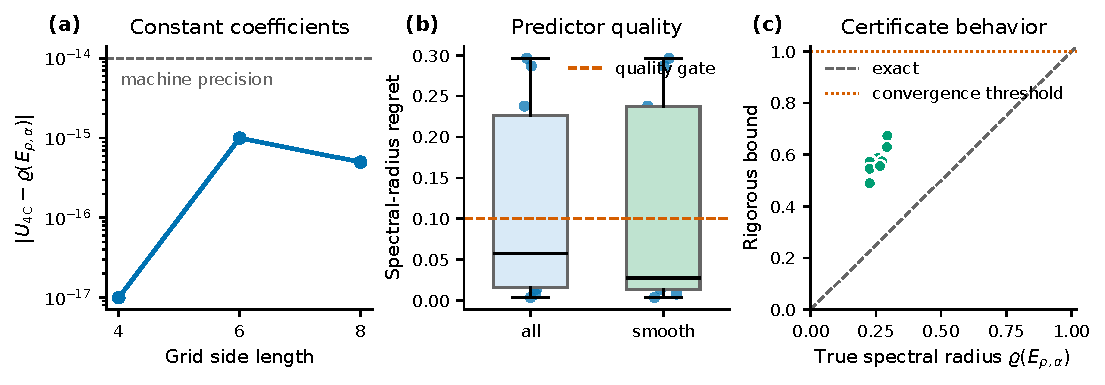
\includegraphics[width=.98\linewidth]{../figures/algebraic_validation.pdf}
\caption{Validation of the four-corner reduction and predictor.
\textbf{(a)} Constant-coefficient periodic systems satisfy the attained
Cartesian-product assumptions; direct eigendecomposition of the full reduced
matrix agrees with $U_{\rm 4C}$ to machine precision.
\textbf{(b)} Spatially varying optical-flow Hessians violate commutativity.
The horizontal axis is the normalized commutator
$\chi=\norm{HG-GH}_2/(\norm H_2\norm G_2)$, and the vertical axis is the
spectral-radius regret
$(R_{\rm act}-R_{\rm ora})/R_{\rm ora}$. Marker shapes identify
magnitude-only, orientation-only, abrupt-interface, and random-gradient
constructions; labels give the sinusoidal amplitude $a$ or Gaussian precursor
scale $\sigma$. Lines connect levels within a construction only as visual
guides.}
\label{fig:spectral}
\end{figure}

\subsection{Real registration benchmarks}
\subsubsection{CIMA histology}
The public lung-lesion-3 sample from the CIMA landmark repository
\cite{Borovec2018} comprises five differently stained sections and all ten
unordered pairs.
Images supplied at 5\% scale were converted to a common structural channel and
resized to $256^2$; landmarks supplied at 50\% scale were rescaled for
evaluation only. The problem is diffeomorphic registration of these pairs under
the shared pyramid solver, comparing one-shot four-corner oADMM tuning with
fixed-parameter, residual-balancing, and BB proxy baselines on target
registration error (TRE), iterations, runtime, and discrete Jacobians. TRE is
the Euclidean landmark error after registration.

The external fixed comparator $(\rho,\alpha)=(0.1,1.0)$ was selected using
separate validation images and then held fixed for CIMA and FIRE. Across five order-alternated
repetitions of all ten pairs (50 paired runs), four-corner tuning reduced
median total runtime by 20.1\% (bootstrap 95\% interval 19.4--20.7\%), solver
time by 23.5\%, and iterations by 30.1\%. Selection used 1.16\% of proposed
runtime. Median TRE was $7.33$ pixels (2.02\% of the image diagonal) and
differed by less than $3\times10^{-5}$ pixels from the fixed comparator. The
median landmark-error improvement relative to the unregistered pairs was
36.5\%. No global or interior nonpositive Jacobian was observed. One difficult
stain pair retained TRE above 22 pixels, identifying initialization and
cross-stain representation rather than inner ADMM convergence as the main
failure mode.

\begin{table}[H]
\centering
\caption{CIMA histology registration at $256^2$: medians of iterations and TRE
over ten pairs, and of total time over 50 paired runs.}
\label{tab:cima}
\begin{tabular}{lrrr}
\toprule
Method & Iterations & Time (s) & TRE (px)\\
\midrule
Canonical fixed ADMM $(1,1)$ & 1910.5 & 12.09 & 7.3310\\
Fixed oADMM $(1,1.8)$ & 1129.5 & 7.37 & 7.3308\\
Residual balancing & 1124.5 & 7.40 & 7.3310\\
BB proxy & 435.5 & 3.44 & 7.3306\\
External fixed comparator $(0.1,1.0)$ & 303.5 & 2.53 & 7.3306\\
\textbf{Four-corner one-shot} & \textbf{210.0} & \textbf{2.02} & 7.3306\\
\bottomrule
\end{tabular}
\end{table}

\subsubsection{FIRE retinal registration}
The public FIRE fundus registration benchmark
\cite{HernandezMatas2017}: all 134 landmarked pairs (14~A, 49~P, and 71~S),
converted to a foreground-percentile-normalized green channel and resized to
$256^2$. Landmarks are used only for evaluation. The problem is retinal
diffeomorphic registration under identical phase-correlation initialization,
pyramid, objective, and stopping criteria, with one CPU BLAS/OpenMP thread.
One-shot four-corner tuning is compared with the external fixed comparator, residual
balancing, a safeguarded BB proxy, and fixed oADMM on iterations, runtime, TRE,
and topology.

Across all pairs, median iterations were 245 for one-shot four-corner tuning
and 412 for the external fixed comparator, a paired median reduction of 39.6\%.
Median total times were $4.774$ and $6.680$ seconds, a 34.4\% paired reduction
(bootstrap 95\% interval 30.7--35.7\%); tuning accounted for 1.2\% of proposed
total time. The safeguarded BB proxy required 623.5 iterations and
$9.435$ seconds; the predictor was faster on 94.0\% of pairs, with a median
paired reduction of 51.7\%. Median TRE differed from the fixed pair by
$-1.4\times10^{-5}$ pixels, the maximum absolute difference was
$3.9\times10^{-4}$ pixels, and no method produced a nonpositive Jacobian.

\begin{table}[H]
\centering
\small
\caption{FIRE retinal registration: 134 pairs at $256^2$ under identical
initialization and solver protocol.}
\label{tab:fire}
\begin{tabular}{lrrrr}
\toprule
Method & Iter. & Time (s) & TRE (px) & TRE/diag. (\%)\\
\midrule
External fixed comparator $(0.1,1.0)$ & 412.0 & 6.680 & 5.50178 & 1.51967\\
Residual balancing & 1434.0 & 22.325 & 5.50211 & 1.51976\\
BB proxy & 623.5 & 9.435 & 5.50175 & 1.51966\\
Fixed oADMM $(1,1.8)$ & 1529.5 & 23.471 & 5.50194 & 1.51971\\
\textbf{Four-corner one-shot} & \textbf{245.0} & \textbf{4.774} & 5.50177 & 1.51966\\
\bottomrule
\end{tabular}
\end{table}
Pairwise percentage reductions need not equal percentage differences between
separately reported method medians.

\begin{figure}[H]
\centering
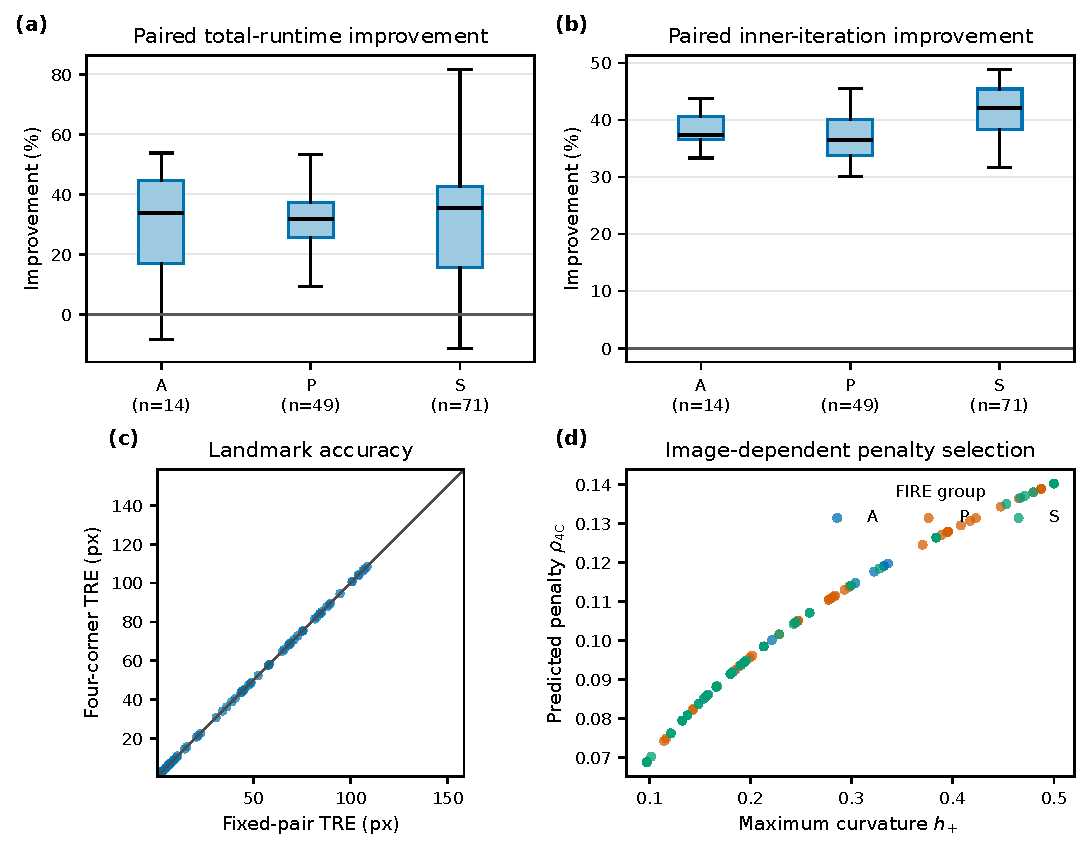
\includegraphics[width=.98\linewidth]{../figures/fire256_headline.pdf}
\caption{FIRE registration at $256\times256$. \textbf{(a)} Pairwise
total-runtime reduction and \textbf{(b)} inner-iteration reduction relative to
the external fixed comparator. \textbf{(c)} Difference in TRE between
four-corner and external fixed parameters. \textbf{(d)} Predicted penalty
versus image-dependent maximum data curvature.}
\label{fig:fire}
\end{figure}

\subsection{One-shot reuse ablation}
On a balanced 18-pair FIRE subset, we compared one-shot reuse of the initial
full-resolution parameter pair with retuning at every pyramid level. Retuning
reduced median inner iterations from 243 to 222 but increased median total time
from $2.651$ to $3.895$ seconds; median parameter-selection time increased from
$0.030$ to $0.110$ seconds. Under this implementation, per-level retuning
therefore traded fewer inner iterations for higher end-to-end runtime. The
reported method uses one-shot reuse; retuning after every outer
Gauss--Newton linearization was not evaluated.

\section{Discussion}\label{sec:discussion}
\subsection{Why four curvature endpoints can suffice}
Separability supplies independent data and regularizer modal coordinates.
Monotonicity along each coordinate line then places the extreme modal values
at endpoint pairs, and convexity of the relaxed magnitude preserves endpoint
maximization.
For registration, the rank-one data Hessian further reduces all data
curvatures to $\nu$ and
$\nu+\mu\max_i\norm{q_i}^2$. The resulting four numbers encode the scale
balance between the data and regularization terms without reference to image
dimension.

\subsection{Transfer beyond the separable model}
In the assembled registration operator, spatially varying data blocks interact
with neighboring regularizer couplings. Smooth coefficient variation can
retain locally meaningful curvature scales even though no global common modal
basis exists. This provides a plausible explanation for the observed transfer
of the surrogate-optimal pair, but not an exact characterization of
$R_{\rm true}$. The predictor omits global orientation interactions among the
rank-one blocks.

\subsection{Expected degradation and computational tradeoff}
Rapid orientation changes, coefficient discontinuities, and strong
noncommutativity increase the mismatch between frozen local models and the
assembled operator. The larger regret in the abrupt-interface experiment is
consistent with this mechanism. More accurate parameter selection can instead
use repeated spectral calculations on the large variable-coefficient
operator. The four-corner predictor occupies the complementary regime: it
uses stronger structural assumptions to make tuning overhead negligible
relative to the solve.

\subsection{Limitations}
The exact theorem requires an attained Cartesian-product joint modal spectrum;
registration uses a noncommuting approximation. The experiments are
two-dimensional and cover FIRE at $256^2$ and one five-image CIMA tissue set at
reduced resolution. The optional certificates are conservative, and the
tested BB proxy represents one safeguarded adaptive implementation. Finally,
the analysis concerns convex linearized subproblems and does not establish
global convergence of the outer nonlinear registration method.

\section{Conclusion}\label{sec:conclusion}
Quadratic oADMM with an attained Cartesian-product joint modal spectrum admits
an exact four-corner characterization of its worst modal contraction. Analytic
relaxation and a finite algebraic penalty candidate set then replace iterative
spectral parameter search. For variable-coefficient registration, local
freezing and the rank-one optical-flow Hessian turn this result into an
inexpensive predictor. FIRE and CIMA experiments show reduced iterations and
runtime with essentially unchanged landmark accuracy and observed topology.
Further work may address tighter noncommuting analysis, volumetric
registration, and related splitting methods.

\section*{Declarations}
\begin{itemize}
\item \textbf{Funding.} No specific funding was received for this work.
\item \textbf{Competing interests.} The authors declare no competing interests.
\item \textbf{Ethics approval and consent to participate.} Not applicable; the
study uses only publicly available, de-identified image datasets.
\item \textbf{Consent for publication.} Not applicable.
\item \textbf{Data availability.} FIRE \cite{HernandezMatas2017} and CIMA
\cite{Borovec2018} are publicly available from their original providers. The
FIRE archive is not redistributed.
\item \textbf{Materials availability.} Not applicable.
\item \textbf{Code availability.} Source code, tests, configurations, processed
JSON and CSV outputs, and preparation and evaluation scripts are available at
\url{https://github.com/xhxuciedu/admm-registration}.
\item \textbf{Author contributions.} Katherine Xie and Jie Wu conducted the
research and wrote and edited the manuscript. Xiaohui Xie conceived the work
and edited the manuscript.
\end{itemize}

\appendix
\section{Proof of the Reduced Cayley Representation}\label{app:reduced}
Let $(v^\star,w^\star,u^\star)$ be a fixed point and write
$\widetilde v^k=v^k-v^\star$, with analogous notation for $w$ and $u$.
Subtracting the fixed-point equations from \eqref{eq:vupdate}--\eqref{eq:uupdate}
removes the affine term $b$. With
\[
P_H=\rho(H+\rho\Id)^{-1},\qquad
P_G=\rho(G+\rho\Id)^{-1},
\]
the homogeneous $v$-update and relaxed variable are
\[
\widetilde v^{k+1}=P_H(\widetilde w^k-\widetilde u^k),\qquad
\widehat{\widetilde v}^{k+1}
=[\alpha P_H+(1-\alpha)\Id]\widetilde w^k
-\alpha P_H\widetilde u^k.
\]
Set
\[
z^k=\widehat{\widetilde v}^{k+1}+\widetilde u^k
=[\alpha P_H+(1-\alpha)\Id]\widetilde w^k
+(\Id-\alpha P_H)\widetilde u^k.
\]
The remaining updates are
$\widetilde w^{k+1}=P_Gz^k$ and
$\widetilde u^{k+1}=(\Id-P_G)z^k$. Thus, for
$s^k=[(\widetilde w^k)^\top,(\widetilde u^k)^\top]^\top$,
\[
s^{k+1}=AB_\alpha s^k,\qquad
A=\begin{bmatrix}P_G\\\Id-P_G\end{bmatrix},\qquad
B_\alpha=
\begin{bmatrix}
\alpha P_H+(1-\alpha)\Id&\Id-\alpha P_H
\end{bmatrix}.
\]
Here $A\in\R^{2N\times N}$ and $B_\alpha\in\R^{N\times2N}$. Sylvester's
determinant identity gives
\[
\det(\lambda\Id_{2N}-AB_\alpha)
=\lambda^N\det(\lambda\Id_N-B_\alpha A).
\]
Hence the nonzero eigenvalues of $AB_\alpha$ and $B_\alpha A$ coincide,
including algebraic multiplicity, and the $2N$-dimensional state map has the
$N$ eigenvalues of $B_\alpha A$ together with $N$ additional zeros.

Direct multiplication yields
\[
\begin{aligned}
B_\alpha A
&=(1-\alpha)\Id+\alpha\{
P_HP_G+(\Id-P_H)(\Id-P_G)\}.
\end{aligned}
\]
Because $P_H=(\Id-C_H)/2$ and $P_G=(\Id-C_G)/2$,
\[
P_HP_G+(\Id-P_H)(\Id-P_G)
=\tfrac12(\Id+C_HC_G).
\]
Therefore
\[
B_\alpha A
=\left(1-\frac{\alpha}{2}\right)\Id
+\frac{\alpha}{2}C_HC_G=E_{\rho,\alpha},
\]
which proves Proposition~\ref{prop:reduced}.

\section{Proof Details for the Four-Corner Theorem}\label{app:corner}
Fix $\rho>0$ and let
$\mathcal R=[h_-,h_+]\times[g_-,g_+]$. The denominators in
\eqref{eq:theta_derivatives} are positive. For fixed $g$, the sign of
$\partial\theta/\partial h$ is the sign of $g-\rho$ and is independent of
$h$; for fixed $h$, the sign of $\partial\theta/\partial g$ is the sign of
$h-\rho$ and is independent of $g$. Consequently, replacing either coordinate
of any point in $\mathcal R$ by a suitable endpoint cannot decrease
$\theta$, and a possibly different endpoint replacement cannot increase it.
Applying this argument successively to both coordinates shows
\[
\theta_{\min}:=\min_{\mathcal R}\theta
=\min_{c\in\operatorname{corners}(\mathcal R)}\theta_c,\qquad
\theta_{\max}:=\max_{\mathcal R}\theta
=\max_{c\in\operatorname{corners}(\mathcal R)}\theta_c.
\]
Thus every attained modal value $t=\theta(h,g;\rho)$ lies in
$[\theta_{\min},\theta_{\max}]$.

For fixed $\alpha>0$, the function
$\phi(t)=|1-\alpha+\alpha t|$ is convex. If
$t=\lambda\theta_{\min}+(1-\lambda)\theta_{\max}$ with
$0\le\lambda\le1$, convexity gives
\[
\phi(t)\le
\lambda\phi(\theta_{\min})+(1-\lambda)\phi(\theta_{\max})
\le\max\{\phi(\theta_{\min}),\phi(\theta_{\max})\}.
\]
Both interval endpoints are corner values, so $\Ufour$ bounds the magnitude
of every modal eigenvalue. If $H$ and $G$ are simultaneously diagonalizable,
$E_{\rho,\alpha}$ is diagonal in their common modal basis and its spectral
radius is the largest modal magnitude. When all four endpoint pairs are
attained common modes, whichever corner realizes the displayed maximum is an
actual eigenmode, proving equality. Without endpoint attainment, the same
argument proves only the rectangular upper envelope.

\section{Proof of Optimal Conditional Relaxation}\label{app:relaxation}
Fix $\rho$ and abbreviate $0\le a\le b\le1$. The four-corner objective is
\[
F(\alpha)=
\max\{|1-\alpha(1-a)|,\ |1-\alpha(1-b)|\},
\qquad 0<\alpha\le2.
\]
If $b=1$, the second endpoint factor equals one for every $\alpha$, while the
first has magnitude at most one for $0<\alpha\le2$ because $0\le a\le1$.
Hence $F(\alpha)=1$ throughout the admissible interval, and every relaxation
is optimal.

Suppose now that $b<1$. The unique unconstrained minimizer is obtained by
equioscillation of the ordered endpoint factors:
\[
1-\alpha(1-a)=-[1-\alpha(1-b)],
\]
which gives $\alpha_0=2/(2-a-b)$. This includes $a=b<1$, for which both
endpoint factors coincide and vanish at $\alpha_0=1/(1-a)$.
The function $F$ is convex and is nonincreasing up to $\alpha_0$, so imposing
$\alpha\le2$ gives $\alpha^\star=\min\{2,\alpha_0\}$.

If $a+b\le1$, then $\alpha_0\le2$, and substitution gives
$F(\alpha^\star)=(b-a)/(2-a-b)$. If $a+b\ge1$, then
$\alpha_0\ge2$ and the constrained optimizer is $\alpha^\star=2$; because
$2b-1\ge1-2a$, its value is $F(2)=2b-1$. The formulas agree when
$a+b=1$.

\section{Proof of Finite Algebraic Selection}\label{app:finite}
For a corner $c=(h_c,g_c)$, write
\[
\theta_c(\rho)=\frac{N_c(\rho)}{D_c(\rho)},\qquad
N_c(\rho)=\rho^2+p_c,\quad
D_c(\rho)=\rho^2+s_c\rho+p_c,
\]
where $s_c=h_c+g_c$ and $p_c=h_cg_c$. Because $\rho>0$ and
$h_c,g_c\ge0$, every $D_c(\rho)=(\rho+h_c)(\rho+g_c)$ is strictly positive.
Identical rational branches are deduplicated.

For distinct branches $i$ and $j$, an intersection satisfies
\[
N_iD_j-N_jD_i
=\rho\big[(s_j-s_i)\rho^2+p_i s_j-p_j s_i\big]=0.
\]
Thus its cleared polynomial has degree at most three (and, after removal of
the inadmissible root $\rho=0$, degree at most two). A relaxation-regime
transition for a possible active pair satisfies
\[
N_iD_j+N_jD_i-D_iD_j=0,
\]
a polynomial of degree at most four.

Let $\mathcal Z$ contain the endpoints of $\mathcal I$ and all roots in
$\mathcal I$ of nonzero pairwise-intersection polynomials. On each connected
component $J$ of $\mathcal I\setminus\mathcal Z$, the strict ordering of all
distinct branches is fixed. Hence there are fixed indices $i$ and $j$ such
that $a=\theta_i$ and $b=\theta_j$ throughout $J$. Partition $J$ further at
the roots of $a+b=1$. On each resulting open interval, the reduced objective
is one of
\[
F_{ij}^{(1)}(\rho)
=\frac{\theta_j-\theta_i}{2-\theta_i-\theta_j},
\qquad
F_j^{(2)}(\rho)=2\theta_j-1.
\]
The denominator in the first regime is at least one and is therefore positive.
When $b=1$ in the second regime, the objective is the constant one and is
handled by the piece endpoints.

After common denominators are cleared, $F_{ij}^{(1)}=P/Q$ with
$\deg P\le3$ and $\deg Q\le4$. Its stationary equation
$P'Q-PQ'=0$ therefore has degree at most six. The stationary equation for
$F_j^{(2)}$ has no larger degree, so six is a common upper bound. These degree
counts also cover coincident curvature endpoints after identical branches
have been removed.

The reduced objective is continuous on the compact interval $\mathcal I$, so
it attains a global minimum. On the closure of each smooth piece, a
nonconstant minimum lies at an endpoint or at an interior stationary point.
If the objective is constant on a piece, either closure endpoint represents
its value. Repeated roots do not create additional pieces. Identically zero
intersection, transition, or stationarity polynomials are discarded; roots
outside $\mathcal I$ and roots associated with inactive branches are also
discarded. The union of the remaining endpoints, intersections, transitions,
and stationary roots is finite and contains a global minimizer. Finally,
evaluating the original objective at this finite superset removes roots made
extraneous by denominator clearing and proves Theorem~\ref{thm:finite}.

\begin{thebibliography}{99}
\bibitem{Ashburner2007}
J. Ashburner, ``A fast diffeomorphic image registration algorithm,''
\emph{NeuroImage}, 38(1):95--113, 2007.
\bibitem{Boyd2011}
S. Boyd, N. Parikh, E. Chu, B. Peleato, and J. Eckstein,
``Distributed optimization and statistical learning via the alternating
direction method of multipliers,'' \emph{Foundations and Trends in Machine
Learning}, 3(1):1--122, 2011.
\bibitem{Borovec2018}
J. Borovec, A. Mu\~noz-Barrutia, and J. Kybic, ``Benchmarking of image
registration methods for differently stained histological slides,'' in
\emph{IEEE ICIP}, pp. 3368--3372, 2018.
\bibitem{ChanElman1989}
T. F. Chan and H. C. Elman, ``Fourier analysis of iterative methods for
elliptic problems,'' \emph{SIAM Review}, 31(1):20--49, 1989.
\bibitem{Ghadimi2015}
E. Ghadimi, A. Teixeira, I. Shames, and M. Johansson, ``Optimal parameter
selection for ADMM: quadratic problems,'' \emph{IEEE Transactions on Automatic
Control}, 60(3):644--658, 2015.
\bibitem{GiselssonBoyd2017}
P. Giselsson and S. Boyd, ``Linear convergence and metric selection for
Douglas--Rachford splitting and ADMM,'' \emph{IEEE Transactions on Automatic
Control}, 62(2):532--544, 2017.
\bibitem{Hering2022}
A. Hering, L. Hansen, T. C. W. Mok, et al., ``Learn2Reg: comprehensive
multi-task medical image registration challenge,'' \emph{IEEE Transactions on
Medical Imaging}, 42(3):697--712, 2023.
\bibitem{HernandezMatas2017}
C. Hern\'andez-Matas, X. Zabulis, A. Triantafyllou, P. Anyfanti, S. Douma, and
A. A. Argyros, ``FIRE: fundus image registration dataset,'' \emph{Journal for
Modeling in Ophthalmology}, 1(4):16--28, 2017.
\bibitem{Kumar2019}
P. Kumar, C. Rodrigo, F. J. Gaspar, and C. W. Oosterlee, ``On local Fourier
analysis of multigrid methods for PDEs with jumping and random coefficients,''
\emph{SIAM Journal on Scientific Computing}, 41(3):A1385--A1413, 2019.
\bibitem{MangBiros2015}
A. Mang and G. Biros, ``An inexact Newton--Krylov algorithm for constrained
diffeomorphic image registration,'' \emph{SIAM Journal on Imaging Sciences},
8(2):1030--1069, 2015.
\bibitem{Rodrigo2017}
C. Rodrigo, F. J. Gaspar, and L. T. Zikatanov, ``On the validity of the local
Fourier analysis,'' arXiv:1710.00408, 2017.
\bibitem{Song2024}
J. Song, W. Lu, Y. Lei, Y. Tang, Z. Pan, and J. Duan, ``Optimizing ADMM and
over-relaxed ADMM parameters for linear quadratic problems,'' in
\emph{Proceedings of AAAI}, 38(8):8117--8125, 2024.
\bibitem{Teixeira2016}
A. Teixeira, E. Ghadimi, I. Shames, H. Sandberg, and M. Johansson, ``The ADMM
algorithm for distributed quadratic problems: parameter selection and
constraint preconditioning,'' \emph{IEEE Transactions on Signal Processing},
64(2):290--305, 2016.
\bibitem{Thorley2021}
A. Thorley, X. Jia, H. J. Chang, et al., ``Nesterov accelerated ADMM for fast
diffeomorphic image registration,'' in \emph{MICCAI}, LNCS 12904, pp. 150--160,
2021.
\bibitem{Vercauteren2009}
T. Vercauteren, X. Pennec, A. Perchant, and N. Ayache, ``Diffeomorphic demons:
efficient non-parametric image registration,'' \emph{NeuroImage},
45(1):S61--S72, 2009.
\bibitem{WienandsJoppich2005}
R. Wienands and W. Joppich, \emph{Practical Fourier Analysis for Multigrid
Methods}. Chapman \& Hall/CRC, 2005.
\bibitem{Wohlberg2017}
B. Wohlberg, ``ADMM penalty parameter selection by residual balancing,''
arXiv:1704.06209, 2017.
\bibitem{Xu2017}
Z. Xu, M. A. T. Figueiredo, and T. Goldstein, ``Adaptive ADMM with spectral
penalty parameter selection,'' in \emph{AISTATS}, PMLR 54:718--727, 2017.
\end{thebibliography}

\end{document}
